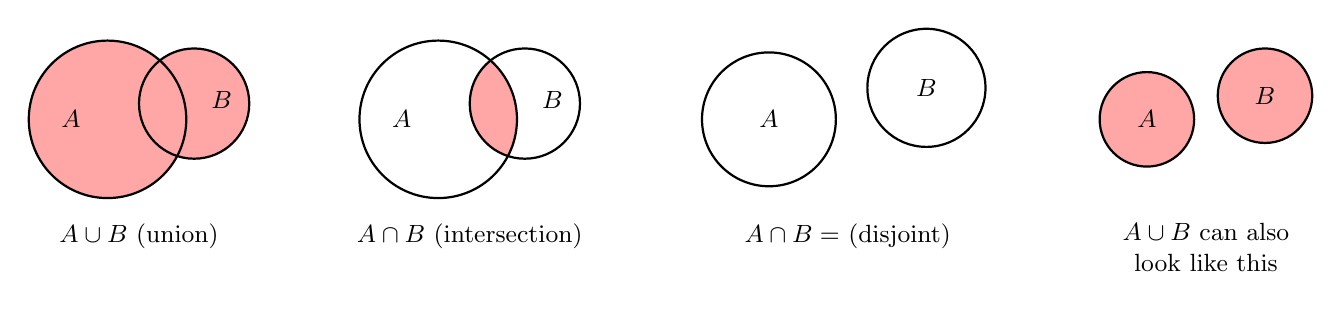
\begin{tikzpicture}[font=\small]
  % union
  \begin{scope}
    \fill[red, fill opacity=0.35] (0,0) circle (1) (1.1,0.2) circle (0.7);
    \draw[thick] (0,0) circle (1) node[left=6pt] {$A$};
    \draw[thick] (1.1,0.2) circle (0.7);
    \node at (1.45,0.25) {$B$};
    \node[below] at (0.4,-1.2) {$A \cup B$ (union)};
  \end{scope}
  % intersection
  \begin{scope}[xshift=4.2cm]
    \begin{scope}
      \clip (0,0) circle (1);
      \fill[red, fill opacity=0.35] (1.1,0.2) circle (0.7);
    \end{scope}
    \draw[thick] (0,0) circle (1) node[left=6pt] {$A$};
    \draw[thick] (1.1,0.2) circle (0.7);
    \node at (1.45,0.25) {$B$};
    \node[below] at (0.4,-1.2) {$A \cap B$ (intersection)};
  \end{scope}
  % disjoint
  \begin{scope}[xshift=8.4cm]
    \draw[thick] (0,0) circle (0.85) node {$A$};
    \draw[thick] (2,0.4) circle (0.75) node {$B$};
    \node[below] at (1,-1.2) {$A \cap B = \varnothing$ (disjoint)};
  \end{scope}
  % union of disjoint sets
  \begin{scope}[xshift=13.2cm]
    \fill[red, fill opacity=0.35] (0,0) circle (0.6) (1.5,0.3) circle (0.6);
    \draw[thick] (0,0) circle (0.6) node {$A$};
    \draw[thick] (1.5,0.3) circle (0.6) node {$B$};
    \node[below, align=center] at (0.75,-1.2) {$A \cup B$ can also\\look like this};
  \end{scope}
\end{tikzpicture}
